\documentclass[tikz,border=6pt]{standalone}
\usepackage{tikz}
\usetikzlibrary{arrows.meta}
\definecolor{nebula}{HTML}{6366F1}
\definecolor{spark}{HTML}{14B8A6}
\definecolor{ink}{HTML}{334155}
\begin{document}
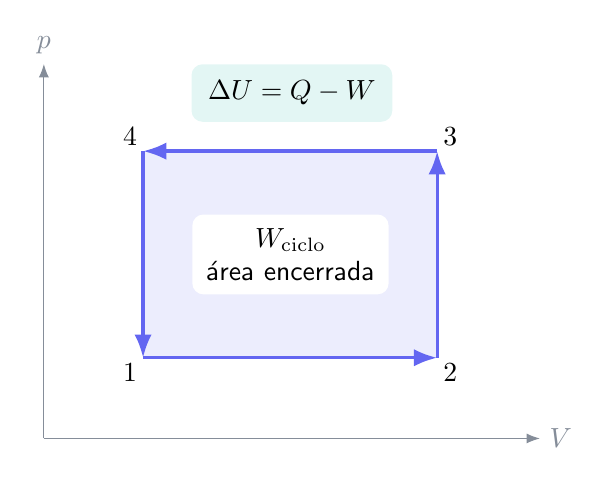
\begin{tikzpicture}[font=\sffamily,>=Latex,x=.9cm,y=.82cm]
  \draw[->,ink!60] (0,0)--(7,0) node[right] {$V$};
  \draw[->,ink!60] (0,0)--(0,5.8) node[above] {$p$};
  \fill[nebula!12] (1.4,1.25) rectangle (5.55,4.45);
  \draw[very thick,nebula,->] (1.4,1.25)--(5.55,1.25);
  \draw[very thick,nebula,->] (5.55,1.25)--(5.55,4.45);
  \draw[very thick,nebula,->] (5.55,4.45)--(1.4,4.45);
  \draw[very thick,nebula,->] (1.4,4.45)--(1.4,1.25);
  \node[below left,fill=white,inner sep=2pt] at (1.4,1.25) {$1$};
  \node[below right,fill=white,inner sep=2pt] at (5.55,1.25) {$2$};
  \node[above right,fill=white,inner sep=2pt] at (5.55,4.45) {$3$};
  \node[above left,fill=white,inner sep=2pt] at (1.4,4.45) {$4$};
  \node[align=center,fill=white,rounded corners=4pt,inner sep=5pt] at (3.48,2.85) {$W_{\rm ciclo}$\\\'area encerrada};
  \node[fill=spark!12,rounded corners=4pt,inner sep=6pt] at (3.5,5.35) {$\Delta U=Q-W$};
\end{tikzpicture}
\end{document}
